\subsection{Plotting a discrete response: Easy smoothing with \PROC{GPLOT}}\label{sec:logist-smooth}

For large \Dsets, extensive computations are required to calculate the lowess curve, because a weighted least squares regression is performed
for each observation.%
\footnote{In \sasver{7}, the \macro{LOWESS} uses the \proc{LOESS}
to perform the calculations, avoiding this difficulty.
In prior versions, use the \mparm{STEP=}{LOWESS} for large \Dsets.
The \mparm{STEP=}{LOWESS} sets a step size for successive
$x$ values.  When \pname{STEP>1}, the macro performs the regression at
every \pname{STEP}-th value of $x$, and uses predicted values from
    that regression for intermediate points.}
A simple alternative, which is often sufficient, is to use the
\pname{SM}\emph{nn} spline smoother provided by the
\pname{INTERPOL} option of the \stmt{SYMBOL}{GPLOT}.
The following example illustrates this technique and the importance
of smoothing.

\begin{Example}[titanic4]{Survival on the \emph{Titanic}}
The \emph{Titanic} data, discussed in \exref{ex:titanic},
included all passengers and crew, but categorized age as either
child or adult.
The data used here lists 1313 passengers by name, and includes the
actual age for 633 of these.
These data were derived from the ``Encyclopedia Titanica''
web site \citep{Hand:97}. They are based on the \emph{Titanic} Passenger List
originally published by \citet{Findlay:86}, and updated
by members of various \emph{Titanic} historical societies and internet
collaborators.
We examine here the relation of sex and class to actual age for these
passengers.

The \Dset\ \pname{titanic2} contains the variables
\pname{SEX}, \pname{CLASS},
\pname{AGE}, \pname{BOAT}, \pname{NAME}, and the 0/1 variable
\pname{SURVIVED}.
A simple, but effective plot of survival probability against age
for men and women is produced just by plotting
\pname{SURVIVED * AGE = SEX}, using \pname{INTERPOL=SM70}
on the \stmt{SYMBOL}{GPLOT}.
The numeric value in \pname{SM}\emph{nn} establishes the relative
weighting of criteria for approximating the points versus
smoothness, with larger values giving a smoother curve.
For binary responses, values in the range 50--90 appear to work
reasonably well.

The following statements produce the left panel in \figref{fig:psurvive12}.
(The \Dstp\ \pname{LABEL}, producing labels for the curves
is not shown to conserve space.)
Similar statements, plotting \pname{SURVIVED * AGE = CLASS}
produce the graph shown in the right panel of \figref{fig:psurvive12}.
\begin{listing}
proc sort data=titanic2;
   by age;

proc gplot data=titanic2;
   where (age^=.);
   plot survived * age = sex /
       anno=label vm=1 hm=1 vaxis=axis1 haxis=axis2 nolegend frame;
   symbol1 i=sm70 v=square   h=1.9 c=red;
   symbol2 i=sm70 v=triangle h=1.9 c=blue;
   axis1 order=(0 to 1 by .2) label=(a=90) offset=(3) value=(h=1.6);
   axis2 offset=(3) value=(h=1.6);
\end{listing}
%% two subfig side-by-side
\begin{figure}[htb]
 \begin{minipage}[t]{.49\linewidth}
  \includegraphics[width=1\linewidth]{ch6/fig/psurvive1}
 \end{minipage}%
 \hfill
 \begin{minipage}[t]{.49\linewidth}
  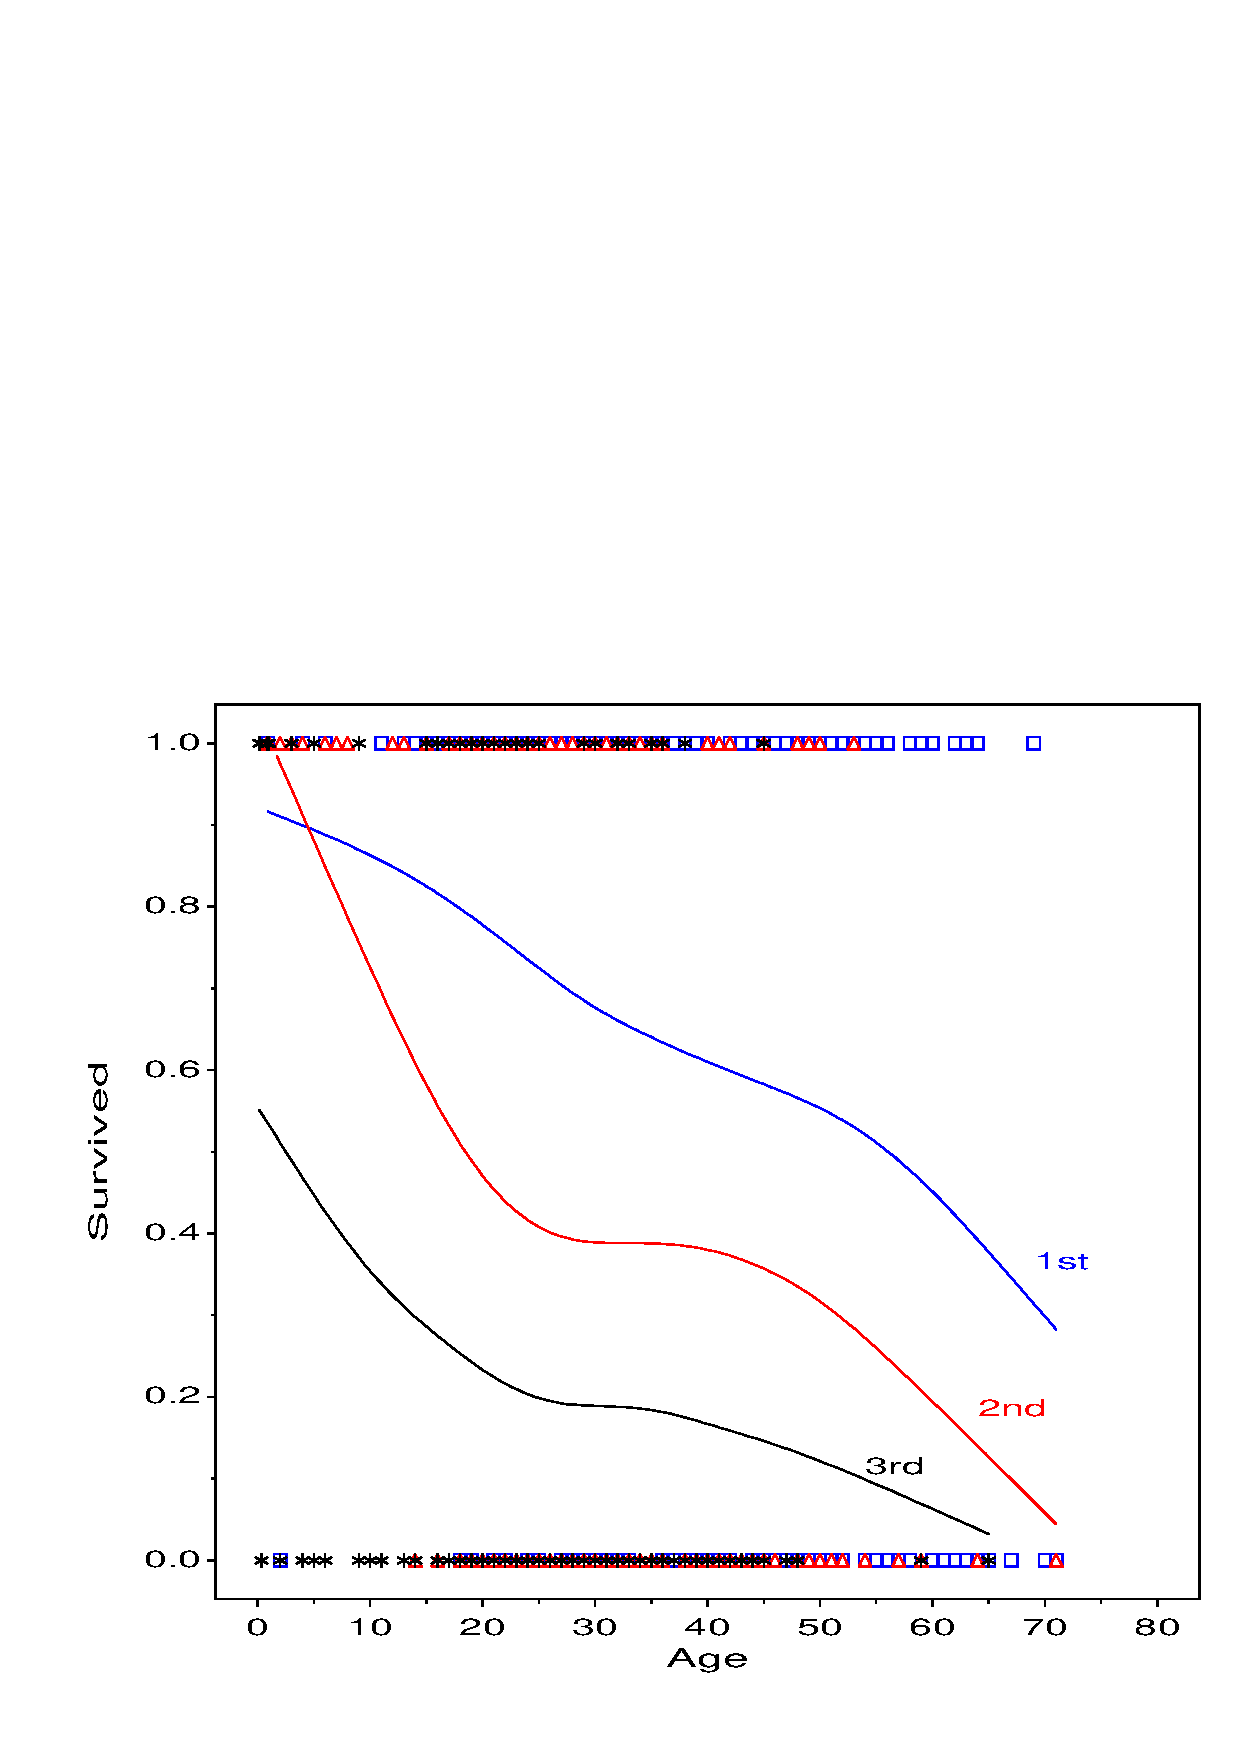
\includegraphics[width=1\linewidth]{ch6/fig/psurvive2}
 \end{minipage}
 \caption[Survival probability vs.\  age by sex (left), and by class (right), for passengers on the \emph{Titanic}]{Survival probability vs.\  age by sex, and by class, for passengers on the \emph{Titanic} whose age is recorded.
 Plot symbols show the individual observations.  These graphs are misleading because the effects of sex vary with class.}\label{fig:psurvive12}
\end{figure}

The actual binary responses, shown by the plotting symbols at
0 and 1 are not very informative here, because age is also discrete
(recorded to the nearest year) and many points are
overplotted.
Jittering the points would help somewhat, but would introduce some bias in
the smoothing.
The smoothed curves are highly suggestive, however,
and give a much more detailed view than our earlier analyses based
on the binary age classification.

For females, probability of survival increases steadily with age.
For males, however, the probability of survival drops precipitously with
age, levels off through middle age, then declines again for the
oldest men.
The smoothed curves in the right panel show similar cubic trends
with age for 2nd and 3rd class passengers.

It is tempting to speculate that these cubic curves reflect
preferential treatment towards boys and
greater chivalry, or perhaps decreased will to survive, on the part of
older men.
Such speculations would be dead wrong, however,
because they falsely assume that sex and class do not interact,
and that the distributions of age (as recorded in this data)
are roughly the same for all sex--class groups.

%% two subfig side-by-side
\begin{figure}[htb]
 \begin{minipage}[t]{.49\linewidth}
  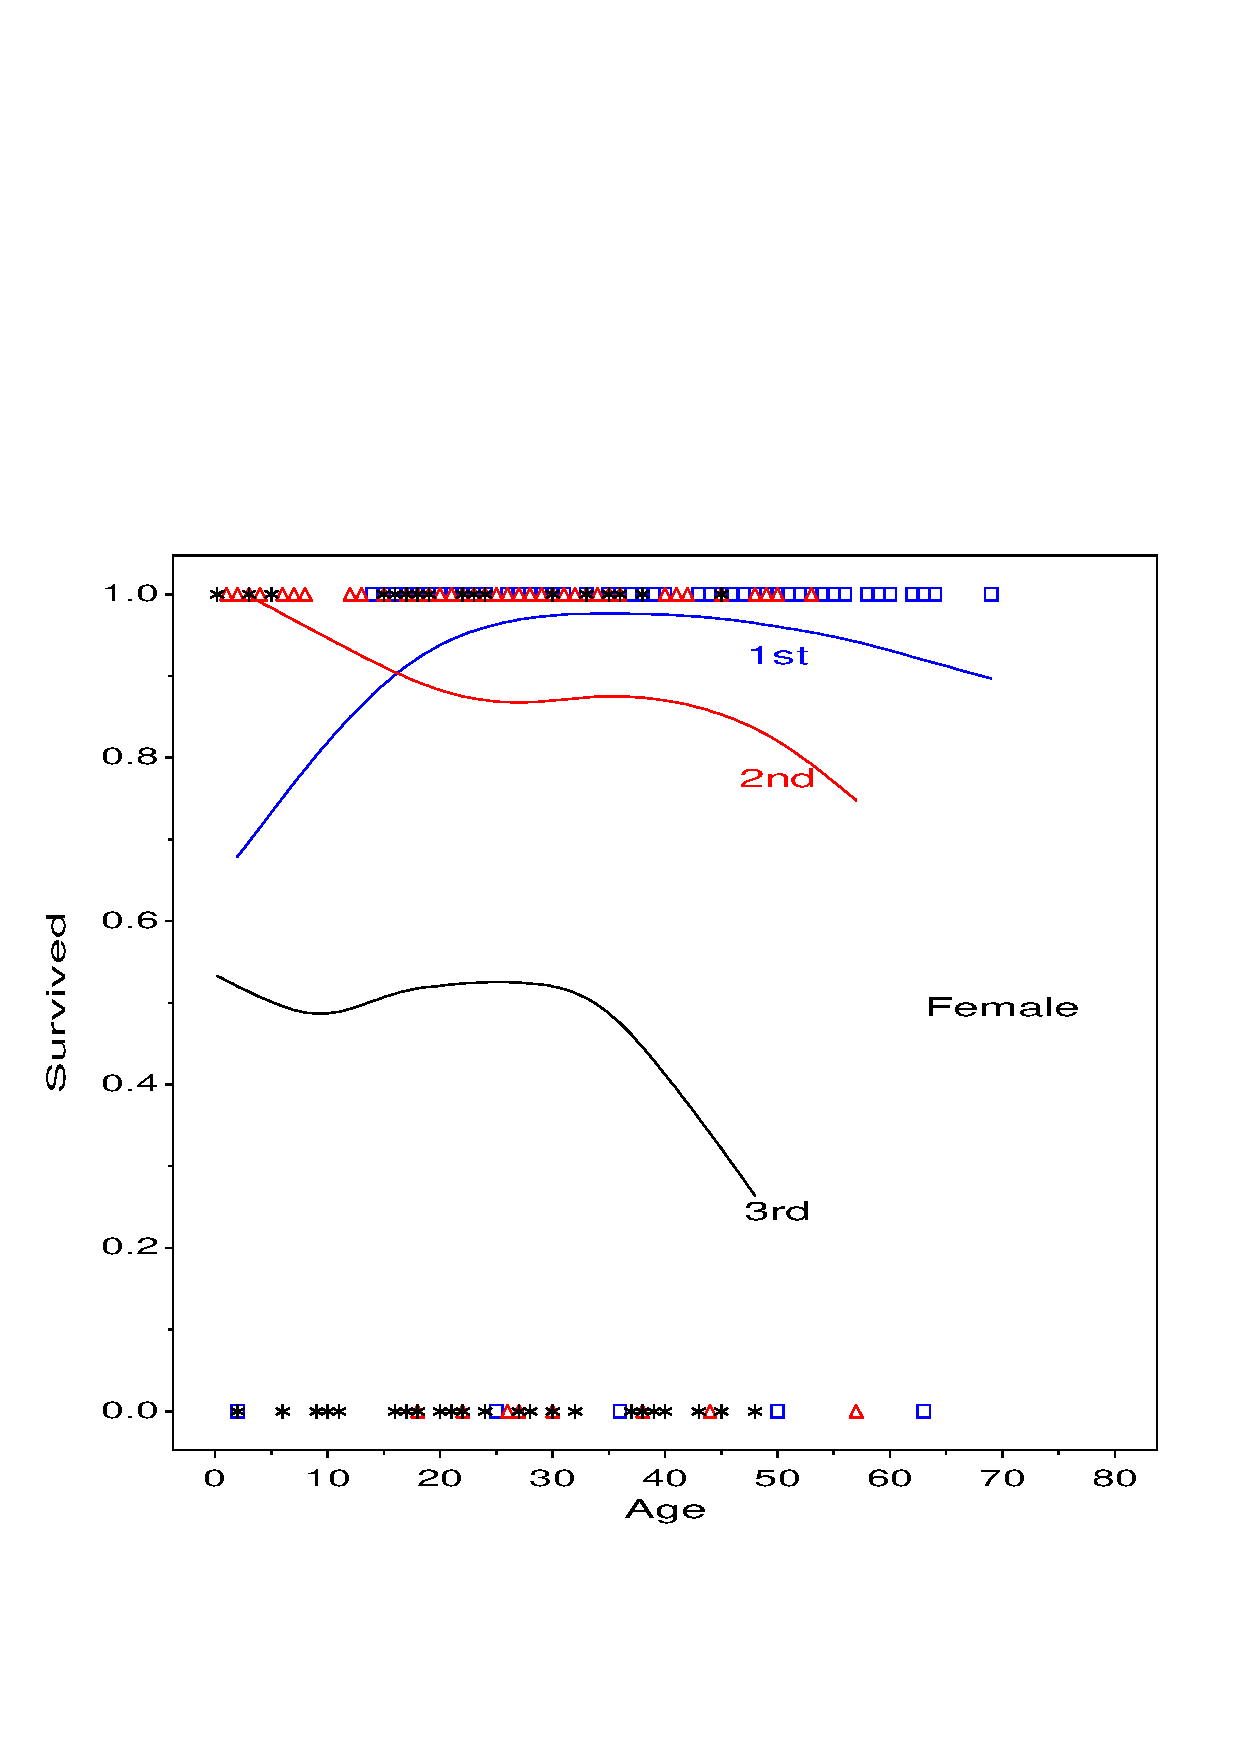
\includegraphics[width=1\linewidth]{ch6/fig/psurvive3}
 \end{minipage}%
 \hfill
 \begin{minipage}[t]{.49\linewidth}
  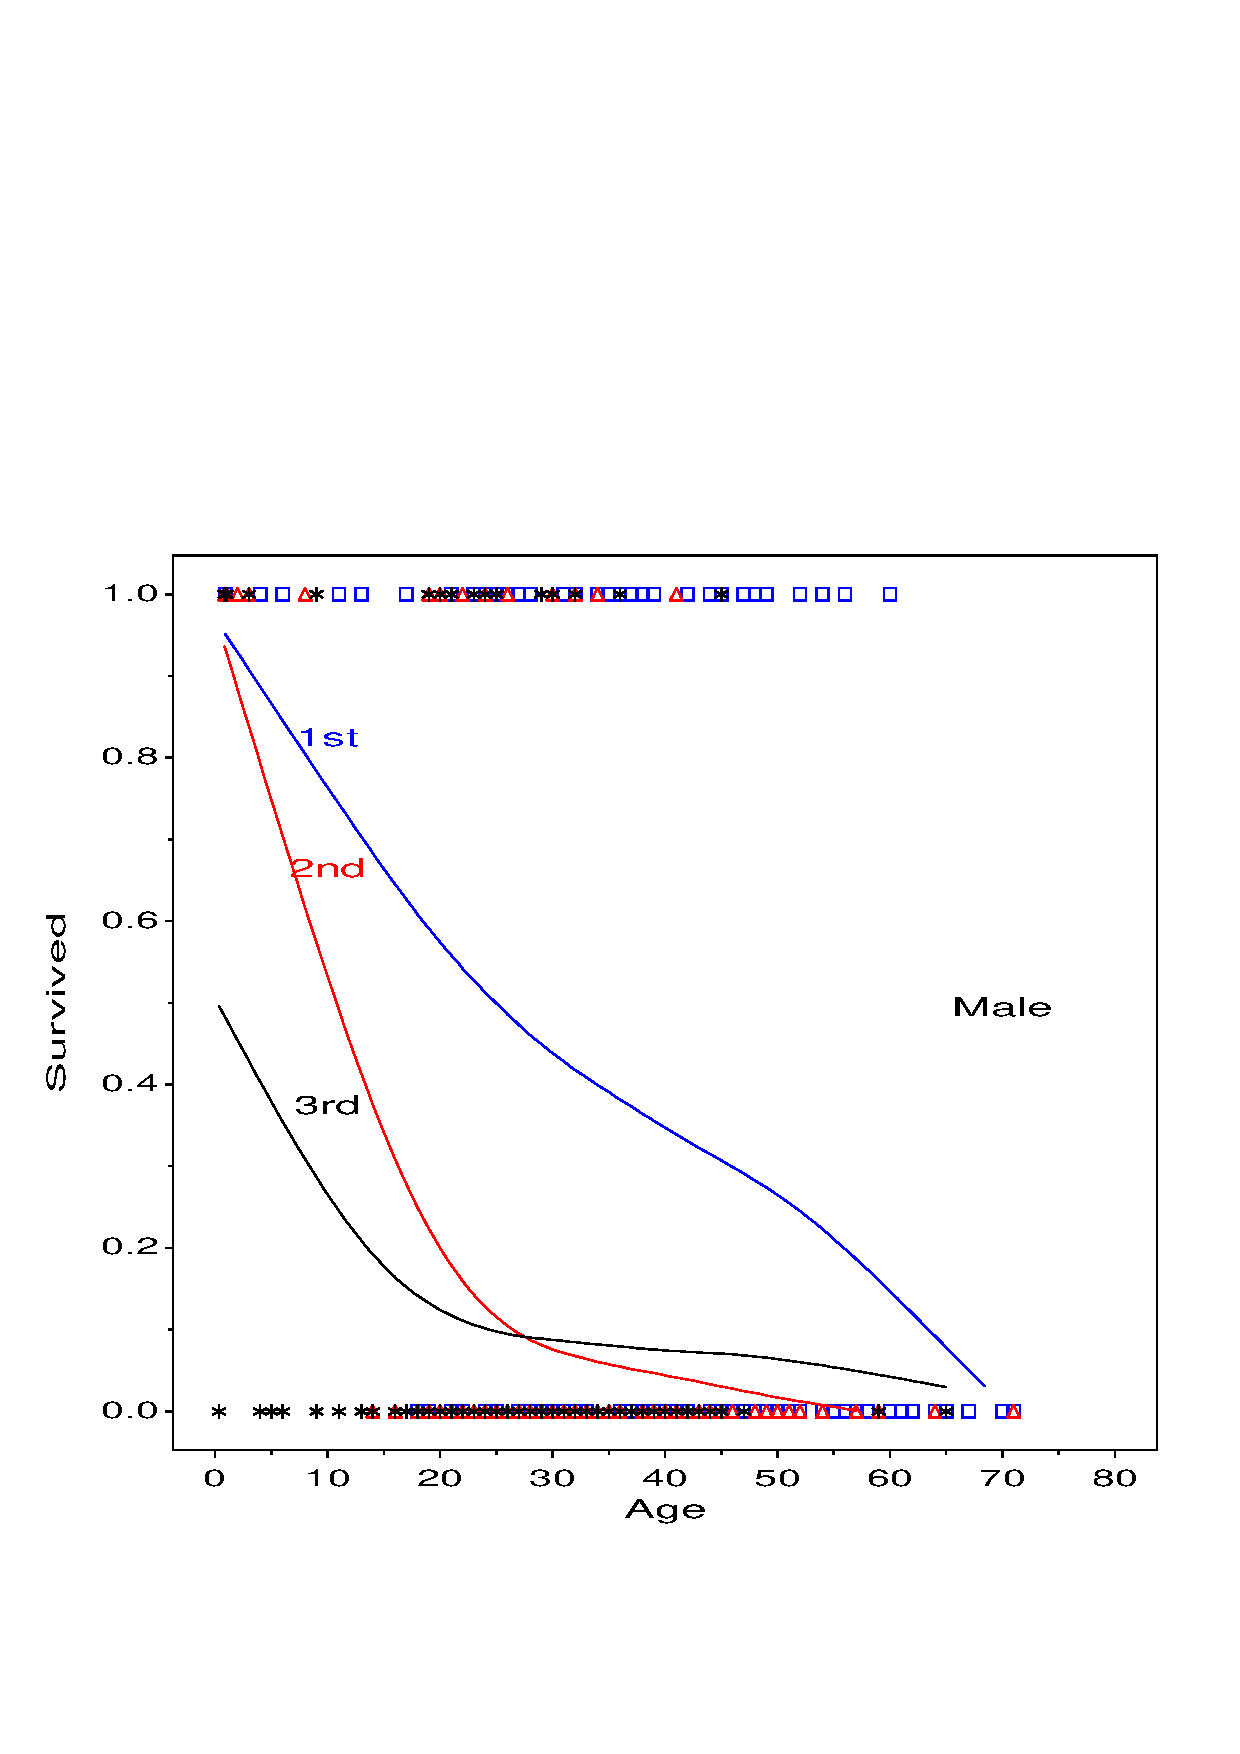
\includegraphics[width=1\linewidth]{ch6/fig/psurvive4}
 \end{minipage}
 \caption{Survival probability vs.\  age by sex--class, for passengers on the \emph{Titanic}}\label{fig:psurvive34}
\end{figure}

We can see that both assumptions are wrong by making separate graphs
for men and women.
These graphs, shown in \figref{fig:psurvive34}, are drawn
using a \stmt{BY}{GPLOT} and smoothing with the \pname{SM}
interpolation method:
\begin{listing}
goptions hby=0;
proc gplot data=titanic2 uniform;
   where (age^=.);
   plot survived * age = class /
      anno=label vm=1 hm=1 vaxis=axis1 haxis=axis2 nolegend frame;
   by sex;
    symbol1 i=sm70 v=square   h=1.9 c=blue;
    symbol2 i=sm70 v=triangle h=1.9 c=red;
    symbol3 i=sm70 v=star     h=1.9 c=black;
\end{listing}
From \figref{fig:psurvive34} it appears that survival of women actually
decreases with age in 2nd and 3rd class; the increasing overall curve
for women in \figref{fig:psurvive12} is due to the greater prevalence of
older women in 1st class, who were more likely to survive.
Among men, it now appears that survival decreases approximately linearly
in 1st class, and much more sharply in the other classes.
However, we must remember that we are just smoothing raw data here; an adequate fitted
model generally provides better smoothing
and simplification.

\end{Example}
